%
%   Chapter Experiment
%
%   Qing-Cheng Li (r01922024 at csie dot ntu dot edu dot tw)
%   R.O.C.103.07
%
\chapter{實驗結果與分析}
\label{c:exp}

本章節進行了以樣式偵測特性的實驗,
以Wikipedia的文章作為模擬內容串流文件、
以YAGO的資料作為答案、
以PATTY提供的樣式對Wikipedia的文章進行偵測。
並介紹評估的標準以及對實驗結果的分析。

\section{測試資料集}
\label{s:dataset}

為了模擬內容串流文件,
本研究以Wikipedia的條目文章作為內容串流中的文件,
自2013年3月的Wikipedia Dumps\footnote{http://dumps.wikimedia.org/}擷取文件。

由於一開始並無文件中包含哪些實體特性的正確資料,
而YAGO的YAGO Facts提供了<subject, property, object>的資訊,
因此我們使用YAGO Facts的propety作為參考答案,
並將subject連結至Wikipedia的文章,
這樣就有每篇文件具有哪些特性的參考答案。

樣式則是使用PATTY提供的樣式釋義,其包含了知識庫定義的關係,
即本研究擬偵測之實體特性,以及可用以表達該特性之樣式集。
實驗採用的是其中的YAGO關係(YAGO Relations),一共有25組關係,
但其中一組關係(YAGO:Produced)在YAGO中沒有找到對映的Wikipedia條目,
因此僅對餘下24組關係進行實驗。

接下來只留下存在這24種特性的Wikipedia條目,
為了防止YAGO Facts中存在某特性但文章中卻根本沒有提及的狀況發生,
我們只留下<subject,property,object>中subject條目內有出現object字詞片段的特性留下,
若object內的字根本沒有出現在文章中,則捨去這個特性。
經過處理後,最後共有334,469篇條目作為測試資料集,
表\ref{t:yago-instance}顯示了各個特性在測試資料集中的數量。

%t:yago-instance
\begin{table}[t]
    \caption{各個特性於測試資料集中出現的文章數}
    \label{t:yago-instance}
    \begin{center}
        \small
        \begin{tabular}{|l|c|}
        \hline
        Property & Number of documents \\
        \hline
        actedIn & 3971\\
        created & 8665\\
        dealsWith & 111\\
        diedIn & 11729\\
        directed & 2036\\
        graduatedFrom & 10474\\
        happenedIn & 1792\\
        hasAcademicAdvisor & 628\\
        hasCapital & 363\\
        hasChild & 2113\\
        hasWonPrize & 8916\\
        holdsPoliticalPosition & 1190\\
        influences & 869\\
        isCitizenOf & 10974\\
        isKnownFor & 73\\
        isLeaderOf & 1397\\
        isLocatedIn & 216772\\
        isMarriedTo & 3555\\
        isPoliticianOf & 170\\
        livesIn & 7661\\
        participatedIn & 346\\
        playsFor & 42751\\
        wasBornIn & 47141\\
        worksAt & 1981\\
        \hline
        \end{tabular}
    \end{center}
\end{table}


表\ref{t:yago-coverage}統計了在不同的信心值下與不同的樣式歧義下,
樣式的數量以及含有這些樣式的文件總數。
由表中可以看出其實當樣式歧義度超過5之後所涵蓋的文件增長速度已經趨於平緩,
因此本實驗最多將只採用歧義度小於等於5的樣式進行。

%t:yago-coverage
\begin{table}[t]
    \begin{center}
        \small
        \begin{tabular}{|l||c|c|c|c||c|c|c|c|}
        \hline
        \multirow{2}{*}{歧義度} & \multicolumn{4}{ c|| }{信心值> 0} & \multicolumn{4}{ c| }{信心值> 0.7} \\
        \cline{2-9}
         & 樣式數 & 出現 & 涵蓋文章 & 比例
            & 樣式數 & 出現 & 涵蓋文章 & 比例 \\
        \hline
        1   & 11381 & 7267  & 250737    & 74.97 & 8913  & 5854  & 244888    & 73.22 \\
        2   & 4778  & 2976  & 275736    & 82.44 & 4175  & 2697  & 272395    & 81.44 \\
        3   & 1255  & 886   & 278820    & 83.36 & 1048  & 745   & 274265    & 82.00 \\
        4   & 666   & 503   & 281256    & 84.09 & 600   & 458   & 276782    & 82.75 \\
        5   & 635   & 465   & 283830    & 84.86 & 605   & 442   & 279603    & 83.60 \\
        \hline
        6   & 77    & 64    & 283858    & 84.87 & 68    & 57    & 279648    & 83.61 \\
        7   & 132   & 100   & 284128    & 84.95 & 131   & 100   & 280096    & 83.74 \\
        8   & 49    & 43    & 284275    & 84.99 & 49    & 43    & 280342    & 83.82 \\
        9   & 26    & 25    & 284295    & 85.00 & 26    & 25    & 280385    & 83.83 \\
        10  & 13    & 11    & 284297    & 85.00 & 13    & 11    & 280387    & 83.83 \\
        11  & 12    & 9 & 284299    & 85.00 & 12    & 9 & 280391    & 83.83 \\
        12  & 2 & 2 & 284299    & 85.00 & 2 & 2 & 280391    & 83.83 \\
        13  & 0 & 0 & 284299    & 85.00 & 0 & 0 & 280391    & 83.83 \\
        14  & 2 & 2 & 284299    & 85.00 & 2 & 2 & 280391    & 83.83 \\
        15  & 0 & 0 & 284299    & 85.00 & 0 & 0 & 280391    & 83.83 \\
        16  & 0 & 0 & 284299    & 85.00 & 0 & 0 & 280391    & 83.83 \\
        17  & 3 & 3 & 284299    & 85.00 & 3 & 3 & 280391    & 83.83 \\
        \hline
        總計 & 19031 & 12356    & -- & --   &15647 &10448 & -- & -- \\
        \hline
        \hline
        \multirow{2}{*}{歧義度} & \multicolumn{4}{ c|| }{信心值> 0.8} & \multicolumn{4}{ c| }{信心值> 0.9} \\
        \cline{2-9}
         & 樣式數 & 出現 & 涵蓋文章 & 比例
            & 樣式數 & 出現 & 涵蓋文章 & 比例 \\
        \hline
        1   & 5951  & 4029  & 222371    & 66.48 & 1879  & 1121  & 155402    & 46.46 \\
        2   & 2328  & 1697  & 251552    & 75.21 & 316   & 206   & 163265    & 48.81 \\
        3   & 683   & 487   & 258715    & 77.35 & 187   & 110   & 170820    & 51.07 \\
        4   & 473   & 355   & 261633    & 78.22 & 67    & 47    & 171978    & 51.42 \\
        5   & 278   & 243   & 262321    & 78.43 & 18    & 16    & 173397    & 51.84 \\
        \hline
        6   & 50    & 43    & 262364    & 78.44 & 10    & 8 & 173457    & 51.86 \\
        7   & 52    & 41    & 262452    & 78.47 & 12    & 8 & 174396    & 52.14 \\
        8   & 13    & 15    & 263419    & 78.76 & 2 & 2 & 174476    & 52.17 \\
        9   & 12    & 12    & 263514    & 78.79 & 8 & 8 & 175287    & 52.41 \\
        \hline
        總計    & 9840  & 6922  & --  & --  & 2499  & 1526  & --  & -- \\
        \hline
        \end{tabular}
        \caption{樣式總數量、出現數量、涵蓋文章與比例於不同信心值之統計}
        \label{t:yago-coverage}
    \end{center}
\end{table}


由於資料集內的Wikipeida條目皆是描寫實體,
在假設文章的內容都是以描寫該實體的前提下,
可以利用YAGO Simple Types作為該文描述實體之類型,
搭配樣式的領域(Domain)資訊輔助偵測。

而第\ref{c:method}章中所提到需要利用過去的資料進行統計、訓練分類器,
則是將測試資料集分為五等份,以其中四等份作為過去的資料,
並對其進行統計或訓練分類器,
餘下的一份進行測試。

\section{評估標準}
\label{s:eval}
在偵測系統的效率方面,
我們以每顆核心在每分鐘內可以處理多少文件來評估,
以及要達到TREC知識庫加速競賽的每小時處理約100,000篇的規模需要多少運算核心或機器。

在偵測系統的效能方面,
我們希望了解對每一個實體特性,
利用樣式自文章中偵測該特性的效能。
因此,以精確率(Precision)、召回率(Recall)、$F_1$分數($F_1$ Score)進行評估。
精確率公式如式\ref{f:precision},召回率公式如式\ref{f:recall}。

\begin{equation}
    \label{f:precision}
    Precision = \frac{|\{relevant\ documents\}\cap\{retrived\ documents\}|}{|\{retrived\ documents\}|}
\end{equation}

\begin{equation}
    \label{f:recall}
    Recall = \frac{|\{relevant\ documents\}\cap\{retrived\ documents\}|}{|\{relevant\ documents\}|}
\end{equation}

對於一個實體特性,經過偵測之後會有被標為有此特性的文件與無此特性的文件。
其中,相關的文件(Relevant documents)即真正存在該特性之文件;
尋回的文件(Retrived documents)即偵測系統標記為擁有此特性之文件。
精確率評估在尋回的文件之中有多少文件真正存在該特性;
召回率評估在真正擁有該特性的文件中有多少被系統偵測到。

$F_1$分數則是綜合評估精確率與召回率,計算方式如式\ref{f:f1},為精確率與召回率的調和平均。

\begin{equation}
    \label{f:f1}
    F_1\ Score = \frac{2\times Precision \times Recall}{Precision + Recall}
\end{equation}

除了評估個別特性的效能之外,以宏觀平均(Macro Average)及微觀平均(Mirco Average)分別計算精確率與召回率及$F_1$分數來評估整體效能。
以精確率為例,宏觀平均的計算如式\ref{f:macro},
而微觀平均的計算則如式\ref{f:micro}。

\begin{equation}
    \label{f:macro}
    Macro\ Avg\ Precision=\frac{\sum_i^n precision_i}{n}
\end{equation}

\begin{equation}
    \label{f:micro}
    Mirco\ Avg\ Precision=\frac{\sum_i^n |\{relevant\ documents\}_i|\cap|\{retrived\ documents\}_i|}{\sum_i^n |\{retrived\ documents\}_i|}
\end{equation}

\section{實驗結果}
\label{s:result}

\subsection{效率}
在圖\ref{i:process-v2}的偵測流程之中,本實驗將其拆解為兩個部份來評估效能。
前半部份為樣式比對的效率,後半部份為特性消歧義的效率。

樣式比對的效率在時脈為2.5GHz的中央處理器為每顆核心每分鐘592份文件,
特性消歧義的效率在同樣條件下為每顆核心每分鐘2750份文件。
要在一小時內處理100,000文件僅需要3顆核心即可完成。
而本實驗使用一台配備時脈2.5GHz、24核心中央處理器的工作站僅需半小時即可處理完全部約330,000份文件。

\subsection{原始效能}
依照圖\ref{i:process-v2}的流程,
但於樣式篩選的部分僅篩選了無歧義度以及歧義度小於等於5的樣式,
而無特性消歧義的結果如表\ref{t:baseline-1}。
表中左半部是每一個特性使用無歧義度,也就是歧義度為1的樣式,
進行特性偵測的結果,由於沒有歧義問題,所以無需進行特性消歧義。

右半部則使用了歧義度5及更小的樣式,而不進行特性消歧義,
可以看到的結果是,由於沒有進行特性消歧義而的對每篇文章回答盡可能多的特性,
因此召回率提升,但精確率也因此下降,$F_1$分數則因為精確率降太多而變低。

由此也可以看出太寬鬆地依據樣式回報特性會降低效能,
後續的實驗將陸續加入樣式篩選與特性消歧義的方法, 嘗試改善效能。

%t:baseline-1
%\begin{sidewaystable}
\begin{table}
    \begin{center}
        \scriptsize
        \begin{tabular}{|l||c|c|c||c|c|c|}
        \hline
        \multirow{2}{*}{Property} & \multicolumn{3}{ c|| }{歧義度1} & \multicolumn{3}{ c| }{歧義度5無篩選} \\
        \cline{2-7}
        & Precision & Recall & $F_1$ Score & Precision & Recall & $F_1$ Score \\ 
        \hline
        actedIn & 0.04346684 & 0.51633265 & 0.0801835267 & 0.02808748 & 0.7975619 & 0.0542639635\\
        created & 0.08228679 & 0.81709385 & 0.1495162939 & 0.05583113 & 0.95001754 & 0.1054642798\\
        dealsWith & 0.00335447 & 1 & 0.0066865103 & 0.00216425 & 1 & 0.0043191523\\
        diedIn & 0.06224856 & 0.36879393 & 0.1065179958 & 0.05507079 & 0.64684916 & 0.1015001618\\
        directed & 0.03927418 & 0.28666455 & 0.0690836289 & 0.02895369 & 0.94029186 & 0.0561775476\\
        graduatedFrom & 0.14718304 & 0.47521937 & 0.2247556578 & 0.11298864 & 0.78572966 & 0.19756697\\
        happenedIn & 0.13234375 & 0.66757981 & 0.2208961453 & 0.13154836 & 0.67313236 & 0.2200859442\\
        hasAcademicAdvisor & 0.02812044 & 0.43292079 & 0.0528105614 & 0.01292023 & 0.68924446 & 0.0253649808\\
        hasCapital & 0.05295147 & 0.34298641 & 0.0917398184 & 0.00585946 & 0.45816088 & 0.0115709382\\
        hasChild & 0.02842344 & 0.63019974 & 0.0543936048 & 0.01822775 & 0.97241921 & 0.0357847245\\
        hasWonPrize & 0.12120602 & 0.01099484 & 0.0201608491 & 0.09693382 & 0.07378178 & 0.0837878879\\
        holdsPoliticalPosition & 0.03016289 & 0.75982481 & 0.0580224532 & 0.01514724 & 0.89445116 & 0.0297899961\\
        influences & 0.0153143 & 0.82712489 & 0.0300718173 & 0.00816085 & 0.9559357 & 0.0161835407\\
        isCitizenOf & 0.11992498 & 0.12948061 & 0.1245197396 & 0.08785729 & 0.39014472 & 0.1434180488\\
        isKnownFor & 0.00212329 & 0.44639731 & 0.0042264768 & 0.00079513 & 0.93804714 & 0.0015889132\\
        isLeaderOf & 0.04677461 & 0.02328296 & 0.0310901841 & 0.01930836 & 0.469555 & 0.0370914972\\
        isLocatedIn & 0.84517473 & 0.52077778 & 0.6444561087 & 0.77085313 & 0.56178423 & 0.6499189428\\
        isMarriedTo & 0.03827487 & 0.6623392 & 0.0723677924 & 0.02744828 & 0.96646594 & 0.0533805175\\
        isPoliticianOf & 0.01632025 & 0.23554096 & 0.0305254418 & 0.00369108 & 0.7024813 & 0.0073435743\\
        livesIn & 0.07468026 & 0.05527752 & 0.0635304722 & 0.06734495 & 0.44379567 & 0.116943933\\
        participatedIn & 0.02227683 & 0.65485327 & 0.043087894 & 0.02020859 & 0.71510601 & 0.039306398\\
        playsFor & 0.52387168 & 0.51813046 & 0.5209852535 & 0.38285718 & 0.6095533 & 0.4703131662\\
        wasBornIn & 0.28617774 & 0.082453 & 0.1280208655 & 0.25226525 & 0.39620268 & 0.3082594019\\
        worksAt & 0.04388619 & 0.35625107 & 0.078145695 & 0.02095881 & 0.86501083 & 0.040926002\\
        \hline
        Macro Average & 0.11690923 & 0.45085499 & 0.1856725305 & 0.09272841 & 0.70398844 & 0.1638718415\\
        Micro Average & 0.22569929 & 0.4356432 & 0.297347781 & 0.12550728 & 0.56034827 & 0.205080464\\
        \hline
        \end{tabular}
        \caption{僅使用無歧義的樣式與歧義度5篩選之實驗結果}
        \label{t:baseline-1}
    \end{center}
%\end{sidewaystable}
\end{table}


\subsection{樣式篩選}
\subsubsection{信心值}
我們利用PATTY提供的信心值進行樣式的篩選,選定了門檻值分別為0(沒有門檻)、0.7、0.8與0.9,
只使用樣式信心值大於門檻值的樣式進行偵測實驗,其結果的宏觀平均與微觀平均$F_1$分數如圖\ref{i:conf-f1}所示。

\begin{figure}[h]
    \centering
    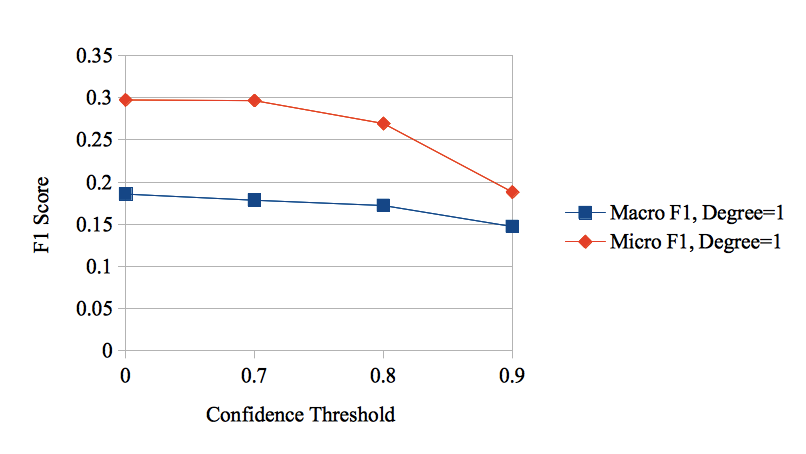
\includegraphics[width=0.85\textwidth]{images/04-conf-f1}
    \caption{無歧義度下F1分數平均隨信心值變化圖}
    \label{i:conf-f1}
\end{figure}

就整體效能而言,設定信心值門檻值並沒有辦法提升系統效能,反而使效能變差。
這是由於設定門檻值後,通過門檻值的樣式數量減少,導致召回率下降太多,
到門檻值為0.9時,有部分的特性(hasCapital, isKnownFor)已經沒有可用的樣式。
但部分的特性$F_1$分數因精確率比較大幅度的提升而略微上昇,表\ref{t:confidence}中,
信心值門檻由0.8昇至0.9,
特性actedIn、created、diedIn、hasAcademicAdvisor、holdsPoliticalPosition、influences、isMarriedTo等的精確率皆有較大幅度的提升。

%t:confidence-f1
\begin{table}[htbp]
\caption{信心值門檻為0.8與0.9各特性效能}
\label{t:confidence}
\begin{center}
\scriptsize
\begin{tabular}{|l||c|c|c||c|c|c|}
    \hline
    \multirow{2}{*}{Property} & \multicolumn{3}{ c|| }{Confidence > 0.8} & \multicolumn{3}{ c| }{Confidence > 0.9} \\
    \cline{2-7}
    & Precision & Recall & $F_1$ Score & Precision & Recall & $F_1$ Score \\ 
    \hline
    actedIn & 0.0490 & 0.3196 & 0.0850 & 0.0833 & 0.1032 & 0.0922 \\
    created & 0.1005 & 0.6682 & 0.1747 & 0.1564 & 0.2208 & 0.1831 \\
    dealsWith & 0.0128 & 0.8935 & 0.0252 & 0.0114 & 0.5805 & 0.0224 \\
    diedIn & 0.0603 & 0.3479 & 0.1028 & 0.1191 & 0.2179 & 0.1540 \\
    directed & 0.0258 & 0.1403 & 0.0436 & 0.1693 & 0.0145 & 0.0267 \\
    graduatedFrom & 0.1022 & 0.2326 & 0.1420 & 0.1129 & 0.0736 & 0.0891 \\
    happenedIn & 0.0638 & 0.1374 & 0.0872 & 0.3010 & 0.0139 & 0.0266 \\
    hasAcademicAdvisor & 0.0288 & 0.3254 & 0.0530 & 0.0468 & 0.2426 & 0.0785 \\
    hasCapital & 0.1117 & 0.0113 & 0.0206 & 0.0000 & 0.0000 & -- \\
    hasChild & 0.0297 & 0.5289 & 0.0563 & 0.0337 & 0.1872 & 0.0572 \\
    hasWonPrize & 0.1212 & 0.0110 & 0.0202 & 0.1193 & 0.0008 & 0.0015 \\
    holdsPoliticalPosition & 0.0350 & 0.7283 & 0.0667 & 0.0437 & 0.4819 & 0.0801 \\
    influences & 0.0195 & 0.7098 & 0.0379 & 0.0616 & 0.3715 & 0.1057 \\
    isCitizenOf & 0.1131 & 0.0790 & 0.0930 & 0.1368 & 0.0293 & 0.0483 \\
    isKnownFor & 0.0024 & 0.4068 & 0.0047 & 0.0000 & 0.0000 & -- \\
    isLeaderOf & 0.0419 & 0.0120 & 0.0187 & 0.0264 & 0.0056 & 0.0092 \\
    isLocatedIn & 0.8806 & 0.4001 & 0.5502 & 0.9066 & 0.1853 & 0.3078 \\
    isMarriedTo & 0.0405 & 0.5531 & 0.0755 & 0.0935 & 0.2915 & 0.1416 \\
    isPoliticianOf & 0.0142 & 0.1527 & 0.0260 & 0.0118 & 0.0720 & 0.0202 \\
    livesIn & 0.0709 & 0.0466 & 0.0563 & 0.0643 & 0.0080 & 0.0143 \\
    participatedIn & 0.0220 & 0.5917 & 0.0423 & 0.0266 & 0.4552 & 0.0503 \\
    playsFor & 0.4966 & 0.2762 & 0.3550 & 0.5432 & 0.0121 & 0.0236 \\
    wasBornIn & 0.3194 & 0.0736 & 0.1196 & 0.3073 & 0.0313 & 0.0569 \\
    worksAt & 0.0435 & 0.1779 & 0.0699 & 0.0404 & 0.0524 & 0.0456 \\
    \hline
    Macro Average & 0.1169 & 0.3260 & 0.1721 & 0.1423 & 0.1521 & 0.1471 \\
    Micro Average & 0.2331 & 0.3190 & 0.2694 & 0.3213 & 0.1328 & 0.1880 \\
    \hline
\end{tabular}
\end{center}
\end{table}



\subsubsection{可信賴度}
透過了過去的統計資料,也就是過去樣式出現時具有特性的比例,對可信賴度進行實驗。
設定了比例為0、0.3與0.5三個門檻值。

實驗的結果呈現如圖\ref{i:reliability-f1},可以看出當門檻值調整至0.3時,
整體系統效能有提升,但再向上調整時就沒有太多上升。
原因是因為當門檻值提升至0.5時,
有些特性(hasCapital、holdsPoliticalPosition、isKnownFor、isLeaderOf、isPoliticianOf、participatedIn)已經沒有可用的樣式。
可信賴度的門檻設定留下了在過去文件中對精確率來說比較好的樣式,
由表\ref{t:reliability}也可以看到精確率隨著門檻值提高而升高,
當然因為使用的樣式越來越少,所以召回率也隨之下降。

\begin{figure}[h]
    \centering
    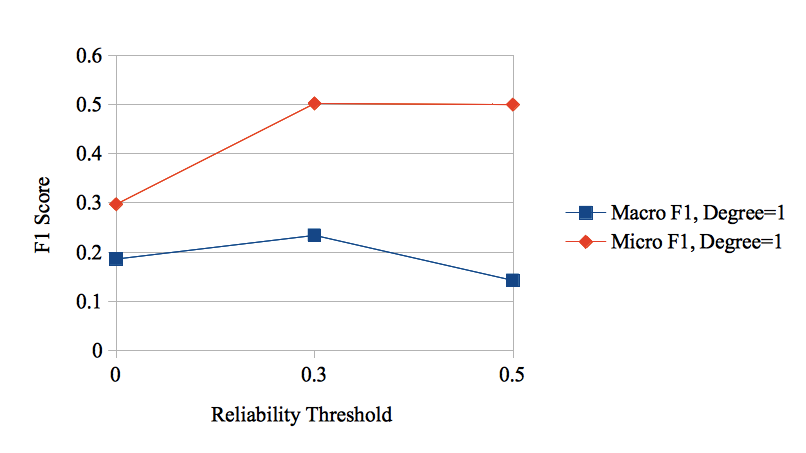
\includegraphics[width=0.85\textwidth]{images/04-reliability-f1}
    \caption{無歧義度下F1分數平均隨可信賴度變化圖}
    \label{i:reliability-f1}
\end{figure}

% t:reliability % TODO
%\begin{table}[htbp]
\centering
\scriptsize
\begin{tabular}{|l|r|r|r|r|r|r|r|r|r|}
\hline
Property & \multicolumn{1}{l|}{Precision} & \multicolumn{1}{l|}{Recall} & \multicolumn{1}{l|}{F1} & \multicolumn{1}{l|}{Precision} & \multicolumn{1}{l|}{Recall} & \multicolumn{1}{l|}{F1} & \multicolumn{1}{l|}{Precision} & \multicolumn{1}{l|}{Recall} & \multicolumn{1}{l|}{F1} \\ \hline
actedIn & 0.0435 & 0.5163 & 0.0802 & 0.4038 & 0.3380 & 0.3680 & 0.5109 & 0.1773 & 0.2632 \\ \hline
created & 0.0823 & 0.8171 & 0.1495 & 0.3122 & 0.5858 & 0.4073 & 0.4790 & 0.4485 & 0.4632 \\ \hline
dealsWith & 0.0034 & 1.0000 & 0.0067 & 0.2499 & 0.7309 & 0.3725 & 0.0250 & 0.0037 & 0.0065 \\ \hline
diedIn & 0.0622 & 0.3688 & 0.1065 & 0.3737 & 0.1130 & 0.1736 & 0.4004 & 0.0145 & 0.0280 \\ \hline
directed & 0.0393 & 0.2867 & 0.0691 & 0.5506 & 0.1305 & 0.2110 & 0.6140 & 0.1133 & 0.1913 \\ \hline
graduatedFrom & 0.1472 & 0.4752 & 0.2248 & 0.3869 & 0.2307 & 0.2891 & 0.4965 & 0.0521 & 0.0943 \\ \hline
happenedIn & 0.1323 & 0.6676 & 0.2209 & 0.5055 & 0.3098 & 0.3842 & 0.7744 & 0.1833 & 0.2964 \\ \hline
hasAcademicAdvisor & 0.0281 & 0.4329 & 0.0528 & 0.3272 & 0.0513 & 0.0887 & 0.0333 & 0.0014 & 0.0027 \\ \hline
hasCapital & 0.0530 & 0.3430 & 0.0917 & 0.0000 & 0.0000 & \multicolumn{1}{l|}{--} & 0.0000 & 0.0000 & \multicolumn{1}{l|}{--} \\ \hline
hasChild & 0.0284 & 0.6302 & 0.0544 & 0.2886 & 0.2432 & 0.2640 & 0.3607 & 0.0267 & 0.0497 \\ \hline
hasWonPrize & 0.1212 & 0.0110 & 0.0202 & 0.3697 & 0.0027 & 0.0054 & 0.5167 & 0.0008 & 0.0015 \\ \hline
holdsPoliticalPosition & 0.0302 & 0.7598 & 0.0580 & 0.0000 & 0.0000 & \multicolumn{1}{l|}{--} & 0.0000 & 0.0000 & \multicolumn{1}{l|}{--} \\ \hline
influences & 0.0153 & 0.8271 & 0.0301 & 0.2137 & 0.2900 & 0.2461 & 0.1952 & 0.0103 & 0.0195 \\ \hline
isCitizenOf & 0.1199 & 0.1295 & 0.1245 & 0.3640 & 0.0118 & 0.0229 & 0.5043 & 0.0039 & 0.0077 \\ \hline
isKnownFor & 0.0021 & 0.4464 & 0.0042 & 0.0000 & 0.0000 & \multicolumn{1}{l|}{--} & 0.0000 & 0.0000 & \multicolumn{1}{l|}{--} \\ \hline
isLeaderOf & 0.0468 & 0.0233 & 0.0311 & 0.0000 & 0.0000 & \multicolumn{1}{l|}{--} & 0.0000 & 0.0000 & \multicolumn{1}{l|}{--} \\ \hline
isLocatedIn & 0.8452 & 0.5208 & 0.6445 & 0.8527 & 0.5206 & 0.6465 & 0.8665 & 0.5188 & 0.6490 \\ \hline
isMarriedTo & 0.0383 & 0.6623 & 0.0724 & 0.3307 & 0.2113 & 0.2579 & 0.5033 & 0.0523 & 0.0947 \\ \hline
isPoliticianOf & 0.0163 & 0.2355 & 0.0305 & 0.1082 & 0.0191 & 0.0324 & 0.0000 & 0.0000 & \multicolumn{1}{l|}{--} \\ \hline
livesIn & 0.0747 & 0.0553 & 0.0635 & 0.3983 & 0.0110 & 0.0214 & 0.4500 & 0.0013 & 0.0026 \\ \hline
participatedIn & 0.0223 & 0.6549 & 0.0431 & 0.1000 & 0.0114 & 0.0204 & 0.0000 & 0.0000 & \multicolumn{1}{l|}{--} \\ \hline
playsFor & 0.5239 & 0.5181 & 0.5210 & 0.6013 & 0.5157 & 0.5552 & 0.6683 & 0.4971 & 0.5701 \\ \hline
wasBornIn & 0.2862 & 0.0825 & 0.1280 & 0.3951 & 0.0588 & 0.1024 & 0.4841 & 0.0083 & 0.0162 \\ \hline
worksAt & 0.0439 & 0.3563 & 0.0781 & 0.3516 & 0.1095 & 0.1670 & 0.4951 & 0.0271 & 0.0514 \\ \hline
Macro Average & 0.1169 & 0.4509 & 0.1857 & 0.3118 & 0.1873 & 0.2340 & 0.3491 & 0.0892 & 0.1421 \\ \hline
Micro Average & 0.2257 & 0.4356 & 0.2973 & 0.7046 & 0.3908 & 0.5027 & 0.8014 & 0.3638 & 0.5004 \\ \hline
\end{tabular}
\caption{TODO}
\label{t:reliability}
\end{table}



\subsubsection{歧義度}
由表\ref{t:yago-coverage}觀察,當歧義度不超過5時所能涵蓋的文件數量就已經非常多了,
因此這裡測試了歧義度由1到5,觀察系統效能的變化結果如圖\ref{i:degree},
由於使用越來越多的樣式,因此召回率快速提高,
但也因此有了歧義問題,使得精確率下降,也讓$F_1$分數下降。
由於有歧義問題,後續的實驗將嘗試消歧義的方法與分析結果。

\begin{figure}[h]
    \centering
    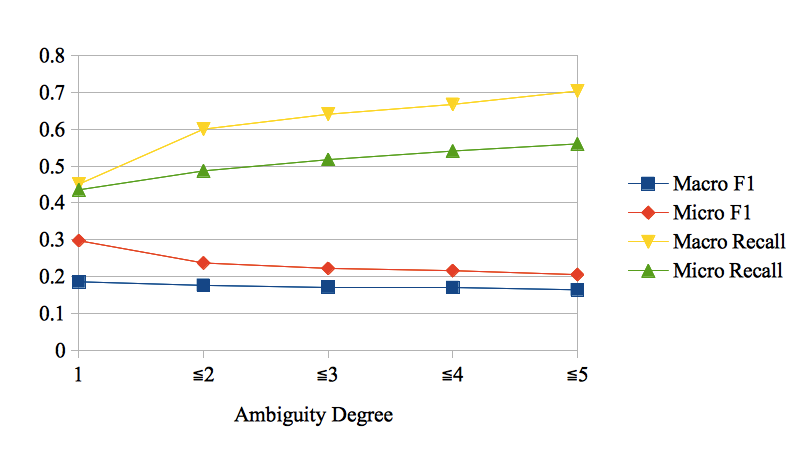
\includegraphics[width=0.85\textwidth]{images/04-degree}
    \caption{F1分數與召回率隨歧義度變化圖}
    \label{i:degree}
\end{figure}

\subsection{特性消歧義}
\subsubsection{實體類型資訊}
\subsubsection{正規化?}
\subsubsection{簡單貝氏分類器}
%\subsecion{}
%錯誤分析
